\documentclass[10pt]{article}

\usepackage{spheric}
%%%TITLE
\title{SPH simulation of drop impact on a hot wall with vaporization effects}
\date{}

%%AFFILIATIONS
\author[1]{Xiufeng YANG}
\author[1]{Song-Charng KONG$^\dagger$}
\affil[1]{Iowa State University, USA}

\author[2]{Moubin LIU$^*$}
\affil[2]{Peking University, China}

\affil[$\relax$]{\email{\dagger}{kong@iastate.edu}, \email{*}{mbliu@pku.edu.cn}}


%%DOCUMENT
\begin{document}

\maketitle

%\SelectedTopics{}

%%PLEASE PUT YOUR ABSTRACT HERE
\begin{abstract}
Drop impact on a hot solid wall is encountered in a number of industrial applications, such as spray cooling of hot surfaces and fuel spray in internal combustion engines \cite{moita2007drop,yang2017simulation}. The process of drop impact on a hot wall involves heat transfer, liquid-gas interface, vaporization, and diffusion of vapor species in the gas phase. Due to the complexity of the problem, it is a challenging work to model the interaction of a droplet and a hot wall.

The purpose of this paper is to present an SPH method for drop impact on a hot wall. By introducing an evaporation model to SPH, the phase change and mass transfer across the liquid-gas interface are simulated. The conservation equation of vapor species is used to simulate the diffusion process of the vapor species in the gas phase. Due to phase change, the mass of an SPH particle at the interface is allowed to change. To avoid large mass difference between SPH particles, particle splitting and merging techniques are developed.

The numerical method is tested by simulating a droplet impacting on a solid wall at different temperatures. The results show that the drop may spread, splash, or breakup on the wall when the wall temperature is lower than the Leidenfrost temperature as shown in figure \ref{fig:9} a-c. However, when the wall temperature is higher than the Leidenfrost temperature \cite{quere2013leidenfrost}, the drop cannot stay on the wall as shown in figure \ref{fig:9} d-f. 


\begin{figure}[!htb]
\centering
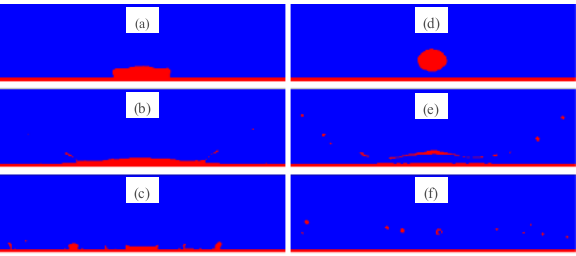
\includegraphics[width=0.95\textwidth]{9-11.png}
\caption{Different outcomes of drop-wall interaction: (a) spread, (b) splash, (c) breakup, (d) rebound, (e) and (f) Leidenfrost phenomena.}\label{fig:9}
\end{figure}

\end{abstract}


%%THE END OF ABSTRACT

\addbib

\end{document}
